\begin{frame}{Coisotropic submanifolds and brackets}
\begin{proposition} If $i: N \hookrightarrow M$ is a $k$-coisotropic submanifold, the subspace of $(k-1)$-forms wich are closed on $N$, $$I_N = \{ [\alpha] \in \Omega^{k-1}_H(M): \,\, d \alpha = 0\, \text{ on } N\}$$ defines a subalgebra of the Lie algebra $\widehat \Omega_H^{k-1}(M).$
\end{proposition}
\pause
\begin{proof}
Let $\widehat{\alpha}, \widehat{\beta} \in \widehat{I}_N.$ Then, there are vector fields $X_\alpha, X_\beta$ satisfying $$\iota_{X_\alpha} \omega = d \alpha, \,\, \iota_{X_\beta} \omega = d \beta.$$ Since $i^\ast d\alpha, i^\ast d\beta = 0,$ we conclude that $X_\alpha, X_\beta$ take values in $(TN)^{\perp, k} \subseteq TN + \ker \flat_1.$ Without loss of generality, we can assume that $X_\alpha$, $X_\beta$ take values in $TN$. Now, since $$\{\widehat{\alpha}, \widehat{\beta}\}^\bullet =  (-1)^{(k-1)} \widehat{ \iota_{X_\alpha \wedge X_\beta} \omega},  i^\ast \left(\iota_{X_\alpha \wedge X_\beta} \omega\right) = 0,$$ concluding that $$\{\widehat{\alpha}, \widehat{\beta}\}^\bullet \in \widehat{I}_N.$$
\end{proof}
\end{frame}

\begin{frame}{Coisotropic reduction}
    Given a $k$-coisotropic submanifold $i: N \hookrightarrow M,$ we have
\begin{proposition} The distribution $x \mapsto (T_x N)^{\perp, k} \cap T_xN \subseteq T_xN$ is involutive.
\end{proposition}
Thus, when it is regular, there exists a foliation consisting of maximal leaves of the distribution, $\mathcal{F}.$ \pause Then,
\begin{theorem} When $N/\mathcal{F}$ admits a smooth manifold structure such that the projection $\pi: N \rightarrow N/\mathcal{F}$ defines a submersion, there exists an unique multisymplectic form $\omega_N$ on $N/\mathcal{F}$ such that $$\pi^\ast \omega_N = i^\ast\omega.$$
\end{theorem}
\alert{What about projection of Lagrangian submanifolds?}
\end{frame}


\begin{frame}{Multisymplectic manifolds of type $(k,r)$} 
\begin{definition}
    Let $L$ be a manifold and $\mathcal{E}$ be a regular distribution on $L$. Define:
$$\bigwedge^k_r L = \{ \alpha \in \bigwedge^k L: \,\, \iota_{e_1 \wedge \cdots \wedge e_r} \alpha = 0, \forall e_1, \dots, e_r \in \mathcal{E}\}.$$
\end{definition}
\pause
\begin{proposition} $(\bigwedge^k_r L, \Omega_L)$ is a non-degenerate multisymplectic manifold, where $\Omega_L$ is (the restriction of the) canononical multisymplectic form.
\end{proposition}
These are the type of multisymplectic manifolds that appear in the study of Classical Field Theories, with $r= 2.$
\end{frame}

\begin{frame}{Multisymplectic manifolds of type $(k,r)$}
\begin{definition} A \alert{multisymplectic manifold} of type $(k,r)$ is a tuple $(M, \omega, W, \mathcal{E}),$ where $(M,\omega)$ is a non-degenerate multisymplectic manifold, $W$ is a regular, integrable, $1$-Lagrangian distribution, and $\mathcal{E}$ is a subbundle of $TM/W$ satisfying
\begin{itemize}
    \item[a)]$\iota_{e_1 \wedge \cdots \wedge e_r} \omega = 0,$ for all $e_i \in TM$ such that $e_i + W \in \mathcal{E};$
    \item[b)] $$\dim \bigwedge^k_r T_qM/ W_q = \dim M.$$
\end{itemize}
\end{definition}
\pause
\begin{theorem} A multisymplectic manifold of type $(k,r)$ $(M, \omega, W, \mathcal{E})$ is locally multisymplectomorphic to $\bigwedge^k_r L$.
\end{theorem}
\end{frame}
\begin{frame}{An example of coisotropic reduction}
    Let $L$ be a smooth manifold, $i: Q \subseteq L$ be a submanifold, and $\mathcal{E}$ be a regular distribution. \pause Then,

    \begin{proposition} $N := \bigwedge^ k_r L \big |_Q$ defines a $k$-coisotropic submanifold, and for $\alpha \in N$, $$\left( T_{\alpha}N\right)^{\perp, k} \cong 0 \oplus \ker i^\ast,$$ where $$i^\ast: \bigwedge^k_r L \rightarrow \bigwedge^k_r Q$$ is the restriction. Here, the vertical forms are taken with respect to $\widetilde{\mathcal{E}} = \mathcal{E} \cap TQ$ (not necessarily of constant rank).
    \end{proposition}
\end{frame}
\begin{frame}{An example of coisotropic reduction}
    \begin{proof} ($r = 0$ for symplicity) To prove the previous equality, we just need to prove it in the linear case $$U \oplus \bigwedge^k L^\ast \subseteq L \oplus \bigwedge^k L^\ast.$$ Let $(v, \alpha) \in (U \oplus \bigwedge^k L^\ast) ^{\perp, k}.$ Then,
    \begin{enumerate}
        \item  $0 = \Omega_L((v, \alpha), (0, \beta), (u_2, 0), \dots, (u_k, 0)) = \beta(v, u_2, \dots, u_k),$ which implies $v = 0$.\pause
        \item $0 = \Omega_L((v, \alpha), (u_1,0), \dots, (u_k, 0)) = \alpha(u_1, \dots, u_k),$ which implies $$\alpha \in \ker i^\ast.$$
    \end{enumerate}
    \end{proof}
\end{frame}

\begin{frame}{An example of coisotropic reduction}
When $\widetilde{\mathcal{E}} = \mathcal{E} \cap Q$ has constant rank, $(TN)^{\perp, k}$ has constant rank and thus, is an involutive distribution. For $x \in Q$, the leaf through $(x, 0) \in N$ is $$\ker \left(i^\ast:\bigwedge^k_r T_x^\ast L \rightarrow \bigwedge^k_r T^\ast_x Q\right).$$ Therefore,
\pause
\begin{theorem} For $N = \bigwedge^k_r L \big |_Q$, where $TQ \cap \mathcal{E}$ has constant rank, $$N/\mathcal{F} \cong \bigwedge^k_r Q.$$ Furthermore, the multisymplectic structure induced on the quotient is the natural multisymplectic structure.
\end{theorem}
\end{frame}

\begin{frame}{Projection of Lagrangian submanifolds (example)}
Define a Lagrangian submanifold through a closed form $$\alpha: L \rightarrow \bigwedge^k_r L.$$ Then, the projection to the quotient $$\pi(\alpha(L) \cap N); \,\, \pi: N \rightarrow N/\mathcal{F}$$ is the image of $$i^\ast\alpha:  Q \rightarrow \bigwedge^k_r Q,$$ which is Lagrangian, because $i^\ast \alpha$ is closed as well.
\pause
\begin{theorem} In our example, Lagrangian submanifold transversal to the vertical distribution reduce to Lagrangian submanifolds.
\end{theorem}
\end{frame}

\begin{frame}{Local characterization of vertical coisotropic submanifolds}
    \begin{definition} Let $(M, \omega, W, \mathcal{E})$ be a multisymplectic manifold of type $(k,r).$ A submanifold $i:N \hookrightarrow M$ is called \alert{vertical} if $W|_N \subseteq TN.$
    \end{definition}
    \pause
    \begin{theorem}[\cite{deleón2024coisotropic}] Let $(M, \omega, W, \mathcal{E})$ be a multisymplectic manifold of type $(k,r)$, $i: N \hookrightarrow M$ be a vertical $k$-coisotropic submanifold, and $j:L \hookrightarrow M$ be a $k$-Lagrangian submanifold complementary to $W$. Then there is a neighborhood $U$ of $L$ in $M$, a submanifold $Q \hookrightarrow L,$ a neighborhood $V$ of $L$ in $\bigwedge^k_r L,$ and a multisymplectomorphism $$\phi: U \rightarrow V$$ satisfying
    \begin{itemize}
        \item[a)] $\phi$ is the identity on $L;$
        \item[b)] $\phi(N \cap U) = \bigwedge^k_r L \big |_Q \cap V.$
    \end{itemize}
    \end{theorem}
\end{frame}
\begin{frame}{Local characterization of Lagrangian submanifolds}
    \begin{theorem}[Normal form of Lagrangian submanifolds \cite{deleon2003tulczyjews}] Let $(M, \omega, W, \mathcal{E})$ be a multisymplectic manifold of type $(k,r)$, $j:L \hookrightarrow M$ be a $k$-Lagrangian submanifold complementary to $W$. Then there is a neighborhood $U$ of $L$ in $M$, a neighborhood $V$ of $L$ in $\bigwedge^k_r L,$ and a multisymplectomorphism $$\phi: U \rightarrow V$$ satisfying
        \begin{itemize}
            \item[a)] $\phi$ is the identity on $L;$
            \item[b)] $\phi( U) =  V.$
        \end{itemize}
        \end{theorem} 
\end{frame}
\begin{frame}{Idea of the proof of local form of coisotropic submanifolds}
    \begin{enumerate}
        \item Take $$\phi: U \rightarrow V$$ the multisymplectomorphism of the previous local form, where $$L \subseteq U \subseteq M; \,\, L \subseteq V \subseteq \bigwedge^k_r L.$$

        \item Define $Q:= \phi(L \cap N).$

        \item Since $\phi$ preserves the vertical distributions, it also preserves their leaves and then, $$\phi(U \cap N) = \bigwedge ^k_r L \big |_ Q \cap V.$$
        \begin{figure}
            \centering
            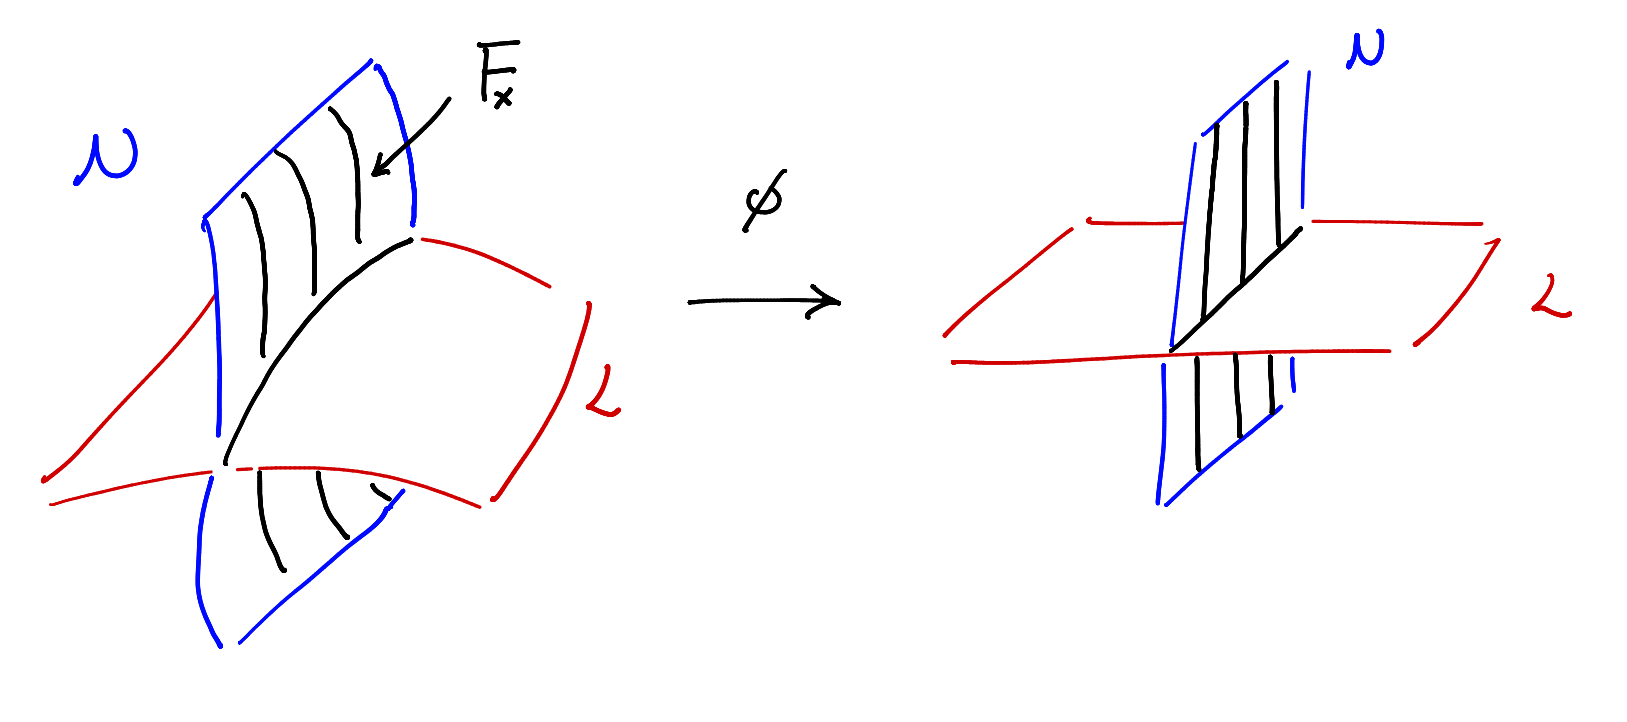
\includegraphics[scale = 0.2]{theorem.PNG}
        \end{figure}
    \end{enumerate}
\end{frame}

\begin{frame}{Lagrangian submanifold projection}
This local characterization allows us to prove:
\begin{theorem}[\cite{deleón2024coisotropic}] Let $(M, \omega, W, \mathcal{E})$ be a multisymplectic manifold of type $(k,r),$ $i: N \hookrightarrow M$ be a vertical $k$-coisotropic submanifold, and $j: L \hookrightarrow M$ be $k$-Lagrangian submanifold complementary to $W$. If $TN / W \cap \mathcal{E}$ has constant rank, so does $(TN)^{\perp, k}$ and we have that, denoting by $\pi: N \rightarrow N/\mathcal{F}$ the canonical projection, \alert{$\pi(L \cap N)$ is Lagrangian in $(N, \omega_N)$}.
\end{theorem}

A general result is not possible, since we can easily find counterexamples.
\end{frame}

\begin{frame}{A counterexample}
Let $L = \langle l_1, l_2, l_3\rangle$ be a $3$-dimensional vector space and define $$V:= L \oplus \bigwedge^2 L^\ast.$$ Let $l^1, l^2, l^3$ be the dual basis induced on $L^\ast$ and denote $$\alpha^{ij} := l^i \wedge l^j.$$ Then $$V = \langle l_1, l_2, l_3, \alpha^{12}, \alpha^{13}, \alpha^{23}\rangle.$$ Let $l^1, l^2, l^3, \alpha_{12}, \alpha_{13}, \alpha_{23}$ be the dual basis. We have $$\Omega_L = \alpha_{12} \wedge l^1 \wedge l^2 + \alpha_{13} \wedge l^1 \wedge l^3 + \alpha_{23}\wedge l^2 \wedge l^3.$$ Define $$N := \langle l_1 + l_2, l_1 + \alpha^{23}, l_2 + \alpha^{13}, l_3, \alpha^{12}\rangle.$$ 

\end{frame}
\begin{frame}{A counterexample}
Then $N$ is a $2$-coisotropic subspace. Indeed, a quick calcultion shows $N^{\perp, 2} = 0$. This implies that the quotient space $N/N^{\perp, 2}$ is (isomorphic to) $N.$ Now, taking as the $2$-Lagrangian subspace $L = \langle l_1, l_2,l_3\rangle$, we have $$L \cap N = \langle l_1 + l_2 , l_3 \rangle.$$ However, this does not define a $2$-Lagrangian subspace of $(N, \Omega_L |_N)$, since $\alpha^{12} \in (N \cap L)^{\perp, 2}$, but $ \alpha^{12} \not \in(L \cap W).$
    
\end{frame}

